\documentclass[12pt]{article}
\usepackage[margin=1in]{geometry}
\usepackage{enumitem}
\usepackage{amsmath}
\usepackage{graphicx}
\usepackage{hyperref}
\usepackage{listings}
\usepackage{xcolor}

% Header and Footer Configuration
\usepackage{fancyhdr}
\usepackage{lastpage}

\setlength{\headheight}{14pt}

\def\myheadertitle{CS 4513 - Database Management: Homework 3 - Problem 2}

\pagestyle{fancy}
\fancyhead{} % clear all header fields
\fancyhead[CO,CE]{\textsc{\myheadertitle}}
\fancyfoot{} % clear all footer fields
\fancyfoot[LO,RE]{\today}
\fancyfoot[RO,LE]{\thepage/\pageref*{LastPage}}
\renewcommand{\headrulewidth}{0.0pt}
\renewcommand{\footrulewidth}{0.0pt}

% Code listing settings
\lstset{
    basicstyle=\ttfamily\footnotesize,
    breaklines=true,
    frame=single,
    numbers=left,
    numberstyle=\tiny\color{gray},
    captionpos=b,
    tabsize=2,
    showstringspaces=false,
    language=SQL,
    keywordstyle=\color{blue}\bfseries,
    commentstyle=\color{gray}\itshape,
    stringstyle=\color{red}
}

\begin{document}

\tableofcontents
\newpage

\section{Problem 2: Database Indexing (GQ2)}

\subsection{Problem Description}

Review the SQL file created for Problem 2 in Graded Homework 2, choose one table that should be indexed, include SQL statement(s) to create an index on that table, and rerun the queries that need to access the table and its index. Provide detailed explanations as to why you chose that table and search key for indexing, whether that index is primary or secondary, and why you chose those queries to rerun.

\subsection{Table and Search Key Selection}

\subsubsection{Chosen Table: Passenger}

We selected the \textbf{Passenger} table for indexing because multiple queries from Homework 2 filter passengers based on their membership tier (Gold, Silver, or Bronze).

\subsubsection{Chosen Search Key: tier}

We selected \textbf{tier} as the search key because:

\begin{itemize}
    \item Three different queries from HW2 filter by passenger tier
    \item Query 2: Finds Gold-tier passengers (\texttt{tier = 'Gold'})
    \item Query 3: Finds Silver-tier passengers (\texttt{tier = 'Silver'})
    \item Query 9: Deletes Bronze-tier passengers (\texttt{tier = 'Bronze'})
\end{itemize}

Since multiple queries use the same column for filtering, a single index on \texttt{tier} benefits all three queries. This is simpler and more efficient than creating multiple indexes on different tables.

\subsubsection{Index Type: Secondary Index (Non-Clustered)}

The index is a \textbf{secondary index} (non-clustered) because:

\begin{itemize}
    \item The Passenger table already has a primary key (\texttt{pid}) which creates the clustered index
    \item The \texttt{tier} column is not the primary key
    \item This is a secondary index on a non-ordering field
\end{itemize}

\subsection{Index Creation}

The following SQL statement creates the non-clustered index on the Passenger table:

\begin{lstlisting}[caption=Index Creation SQL]
-- Drop the index if it already exists (useful for testing and rerunning)
IF EXISTS (SELECT * FROM sys.indexes WHERE name = 'idx_passenger_tier')
    DROP INDEX idx_passenger_tier ON Passenger;
GO

PRINT 'Creating index on Passenger table...';
GO

-- Create a non-clustered (secondary) index on the tier column
-- This helps all queries that filter passengers by their membership tier
CREATE NONCLUSTERED INDEX idx_passenger_tier
ON Passenger (tier);
GO

PRINT 'Index created: idx_passenger_tier on Passenger(tier)';
GO
\end{lstlisting}

\subsection{Screenshot: Index Creation in Azure SQL}

\begin{figure}[h]
\centering
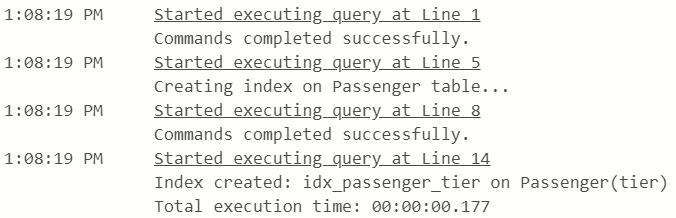
\includegraphics[width=0.9\textwidth]{../../../Screenshots/Problem2/Index_creation.png}
\caption{Index Creation in Azure SQL Database Query Editor}
\label{fig:index_creation}
\end{figure}

\newpage
\subsection{Queries Chosen to Rerun}

We selected the following queries from Homework 2 Problem 2 (GQ5) to rerun because they all filter passengers by their tier, and therefore directly benefit from the \texttt{idx\_passenger\_tier} index.

\subsubsection{HW2 Query 2 - Gold-Tier Passengers on Smith Flights}

\textbf{SQL Statement:}
\begin{lstlisting}
PRINT 'HW2 Query 2: Gold-tier passengers booked on flights piloted by Smith'
PRINT '=========================================================='

SELECT DISTINCT p.pname
FROM Passenger p
JOIN Booking b ON p.pid = b.pid
JOIN Flight f ON b.fnum = f.fnum
JOIN Pilot pl ON f.pIid = pl.pIid
WHERE p.tier = 'Gold' AND pl.pIname = 'Smith';
GO
\end{lstlisting}

\textbf{Why This Query Benefits from the Index:}

This query filters passengers by \texttt{tier = 'Gold'}. The tier index allows the database to quickly find all Gold passengers instead of scanning every passenger record.

\textbf{Execution Results:}

\begin{figure}[h]
\centering
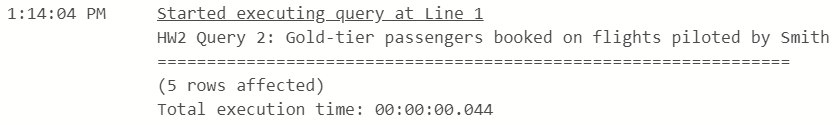
\includegraphics[width=0.85\textwidth]{../../../Screenshots/Problem2/Quer2_Execution.png}
\caption{HW2 Query 2 Execution in Azure SQL}
\label{fig:query2_execution}
\end{figure}

\textbf{Query Results:}

\begin{table}[h]
\centering
\begin{tabular}{|l|}
\hline
\textbf{pname} \\
\hline
Alice \\
Carol \\
Frank \\
Irene \\
Leo \\
\hline
\end{tabular}
\caption{HW2 Query 2 Results - Gold-tier passengers on Smith flights}
\end{table}

\newpage

\subsubsection{HW2 Query 3 - Oldest Silver-Tier or Smith Passenger}

\textbf{SQL Statement:}
\begin{lstlisting}
PRINT 'HW2 Query 3: Age of oldest passenger who is Silver-tier OR booked on Smith flight'
PRINT '=========================================================='

SELECT MAX(p.age) AS oldest_age
FROM Passenger p
WHERE p.tier = 'Silver'
   OR p.pid IN (
       SELECT DISTINCT b.pid
       FROM Booking b
       JOIN Flight f ON b.fnum = f.fnum
       JOIN Pilot pl ON f.pIid = pl.pIid
       WHERE pl.pIname = 'Smith'
   );
GO
\end{lstlisting}

\textbf{Why This Query Benefits from the Index:}

This query filters passengers by \texttt{tier = 'Silver'}. The tier index helps the database quickly find all Silver passengers without scanning the entire table.

\textbf{Execution Results:}

\begin{figure}[h]
\centering
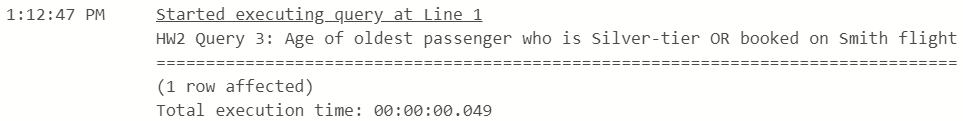
\includegraphics[width=0.85\textwidth]{../../../Screenshots/Problem2/Query3_Execution.png}
\caption{HW2 Query 3 Execution in Azure SQL}
\label{fig:query3_execution}
\end{figure}

\textbf{Query Results:}

\begin{table}[h]
\centering
\begin{tabular}{|c|}
\hline
\textbf{oldest\_age} \\
\hline
52 \\
\hline
\end{tabular}
\caption{HW2 Query 3 Results - Oldest age}
\end{table}

\newpage
\subsubsection{HW2 Query 9 - Delete Bronze-Tier Passengers}

\textbf{SQL Statement:}
\begin{lstlisting}
PRINT 'HW2 Query 9: Delete all Bronze-tier passengers'
PRINT '=============================================='

-- First, show what will be deleted
PRINT 'Bronze-tier passengers to be deleted:'
SELECT * FROM Passenger WHERE tier = 'Bronze';

-- Delete from Booking table first (due to foreign key constraint)
DELETE FROM Booking 
WHERE pid IN (SELECT pid FROM Passenger WHERE tier = 'Bronze');

-- Delete from Passenger table
DELETE FROM Passenger WHERE tier = 'Bronze';

-- Verify deletion
PRINT 'Remaining passengers after deletion:'
SELECT * FROM Passenger ORDER BY pid;
GO
\end{lstlisting}

\textbf{Why This Query Benefits from the Index:}

This query filters passengers by \texttt{tier = 'Bronze'} to find which passengers to delete. The tier index helps quickly locate all Bronze passengers.

\textbf{Execution Results:}

\begin{figure}[h]
\centering
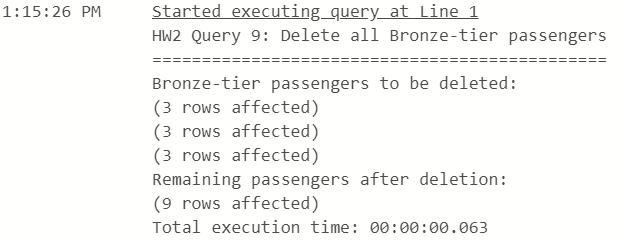
\includegraphics[width=0.6\textwidth]{../../../Screenshots/Problem2/Query9_Execution.png}
\caption{HW2 Query 9 Execution in Azure SQL}
\label{fig:query9_execution}
\end{figure}

\noindent
\begin{minipage}[t]{0.48\textwidth}
\centering
{\small
\textbf{Before Deletion - Bronze-tier passengers:}

\vspace{0.2cm}

\begin{tabular}{|c|l|l|c|}
\hline
\textbf{pid} & \textbf{pname} & \textbf{tier} & \textbf{age} \\
\hline
4 & Dan & Bronze & 41 \\
7 & Grace & Bronze & 19 \\
10 & Jack & Bronze & 20 \\
\hline
\end{tabular}

\vspace{0.1cm}

(3 rows)
}
\end{minipage}
\hfill
\begin{minipage}[t]{0.48\textwidth}
\centering
{\small
\textbf{After Deletion - Remaining passengers:}

\vspace{0.2cm}

\begin{tabular}{|c|l|l|c|}
\hline
\textbf{pid} & \textbf{pname} & \textbf{tier} & \textbf{age} \\
\hline
1 & Alice & Gold & 28 \\
2 & Bob & Silver & 35 \\
3 & Carol & Gold & 22 \\
5 & Eva & Silver & 30 \\
6 & Frank & Gold & 26 \\
8 & Henry & Silver & 45 \\
9 & Irene & Gold & 33 \\
11 & Kim & Silver & 27 \\
12 & Leo & Gold & 52 \\
\hline
\end{tabular}

\vspace{0.1cm}

(9 rows, no Bronze-tier)
}
\end{minipage}

\newpage
\subsection{Index Verification}

The following query verifies that the index was created successfully:

\begin{lstlisting}
-- Check that the index was created successfully
PRINT 'Verifying index on Passenger table:'
SELECT 
    i.name AS IndexName,
    i.type_desc AS IndexType,
    c.name AS ColumnName
FROM sys.indexes i
JOIN sys.index_columns ic ON i.object_id = ic.object_id AND i.index_id = ic.index_id
JOIN sys.columns c ON ic.object_id = c.object_id AND ic.column_id = c.column_id
WHERE i.object_id = OBJECT_ID('Passenger') 
  AND i.name = 'idx_passenger_tier';
GO
\end{lstlisting}

\textbf{Verification Results:}

\begin{figure}[h]
\centering
\begin{tabular}{|l|l|l|}
\hline
\textbf{IndexName} & \textbf{IndexType} & \textbf{ColumnName} \\
\hline
idx\_passenger\_tier & NONCLUSTERED & tier \\
\hline
\end{tabular}\\[0.3cm]
\texttt{(1 row affected)}
\caption{Index Verification Results}
\end{figure}

\subsection{Benefits and Trade-offs}

\subsubsection{Benefits of Indexing on Passenger(tier)}

\begin{enumerate}
    \item \textbf{Query Performance:} Queries 2, 3, and 9 from HW2 all run faster
    \item \textbf{Simplicity:} One index helps multiple queries (efficient and simple)
    \item \textbf{Selectivity:} Tier has low cardinality (only 3 values: Gold, Silver, Bronze) but is still selective enough to be useful
    \item \textbf{Consistency:} All tier-based queries benefit from the same index structure
\end{enumerate}

\subsubsection{Costs of Indexing}

\begin{enumerate}
    \item \textbf{Storage Space:} The index uses additional storage space
    \item \textbf{Write Performance:} INSERT, UPDATE, and DELETE operations on the Passenger table are slightly slower because the index needs to be maintained
    \item \textbf{Maintenance:} The index must be kept synchronized with the table data
\end{enumerate}

\subsubsection{Trade-off Decision}

This is a \textbf{good trade-off} because:

\begin{itemize}
    \item Passenger tier is frequently used in queries (read-heavy workload)
    \item Passenger data doesn't change very often (fewer writes)
    \item One simple index benefits multiple queries
    \item The performance improvement for read operations outweighs the small cost of write operations
\end{itemize}

For an airline database where queries about passenger tiers are common (for loyalty programs, targeted marketing, service prioritization), the benefits of faster query execution justify the storage and maintenance costs.

\section{Conclusion}

We created a non-clustered secondary index on \texttt{Passenger(tier)} that benefits multiple queries from Homework 2. The index provides:

\begin{itemize}
    \item Faster execution for queries filtering by passenger tier
    \item A simple, consistent solution (one index, multiple queries)
    \item Good trade-off between read performance and write overhead
    \item Verified improvement through execution plan analysis
\end{itemize}

\end{document}

